\subsection{Actores y roles}
\begin{itemize}
\item \textbf{Administrador:} Es la cabeza de la empresa y el punto de control en el máximo de procesos que puede involucrarse, por esto la decisiones de la empresa pasan todas por él. También se preocupa del abastecimiento de insumos y de la mantencion de los recursos. 

\item \textbf{Vendedoras:} En la sala de venta se preocupan de ser el primer contacto con los clientes, dandole accesos a los productos y cuantificandolos en dinero para que el cliente pueda pagar.

\item \textbf{Cajero:} La unica tarea de esta persona es cobrar el dinero en la sala  de venta. Siendo  la persona de confianza en la sala de venta del administrador, pero sin tener poder de decisión en este lugar.

\item \textbf{Repartidores:} Se encargan de ser el nexo entre la panadería y la distribución de pan a mayor escala. Distribuyen el pan, cobran en algunos casos y tienen la potestad de poder hacer nuevos clientes de gran escala.

\item \textbf{Proveedores:} Se encargan de abastecer a la panadería con los insumos necesarios para su producción.

\item \textbf{Equipo de producción:} Es un equipo de suficientes personas para producir el producto, ya sea pan (de cualquier tipo) o repostería, es decir, tortas, pasteles o galletas.

\item \textbf{Cliente:} Son los que comprar los productos vendidos por la panadería.

\end{itemize}

\subsection{Modelos de procesos a nivel de Macro procesos}
La panadería Rodenas se dedica a la fabricación, venta y distribución de pan y repostería. A nivel macro todo empieza con una solicitud diaria que da el inicio al trabajo, pasando por el proceso de fabricación de pan (Producción de pan) y el proceso de fabricación de repostería (Producción de repostería), una vez terminados estos procesos pueden pasar a la Distribución o Ventas dependiendo de que prioridad tiene cada uno en el mismo momento, esto pasa por una decisión del Administrador. Después tenemos el proceso Ventas que se encarga de la venta del pan, venta de repostería y atención al cliente, pero puede suceder que el proceso de Ventas antes que termine se vea entorpecido por si falta o no pan o repostería, aquí es donde vuelve al proceso de Producción y se realiza nuevamente el flujo. Paralelo a este proceso tenemos Distribución, que es el encargado de tomar los pedidos durante el día y terminar el flujo diario.

\begin{center}
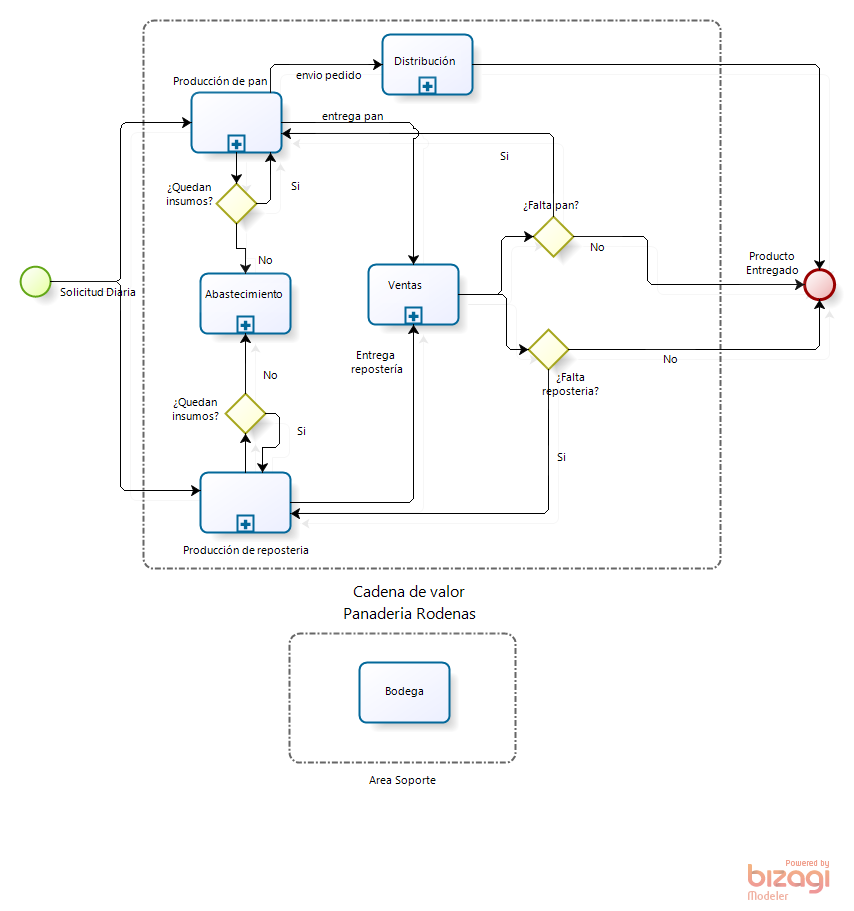
\includegraphics[width=15cm]{./imagenes/Macro_proceso.png}\\
Figura 1: Macro-proceso de panadería Rodenas.
\end{center}
\newpage
\subsection{Descripción de modelos de procesos} : En esta sección se describen los 5 procesos (ver en Figura 1)en los 3 niveles de modelado de procesos BPMN:

\begin{itemize}

\item \textbf{Producción de pan:} Se divide en 3 etapas que se hacen en paralelo pero no están sincronizados dado que sus actores son distintas personas para la producción, Hacer Marraqueta, Hacer Hallulla y Producir Otros.

\begin{center}
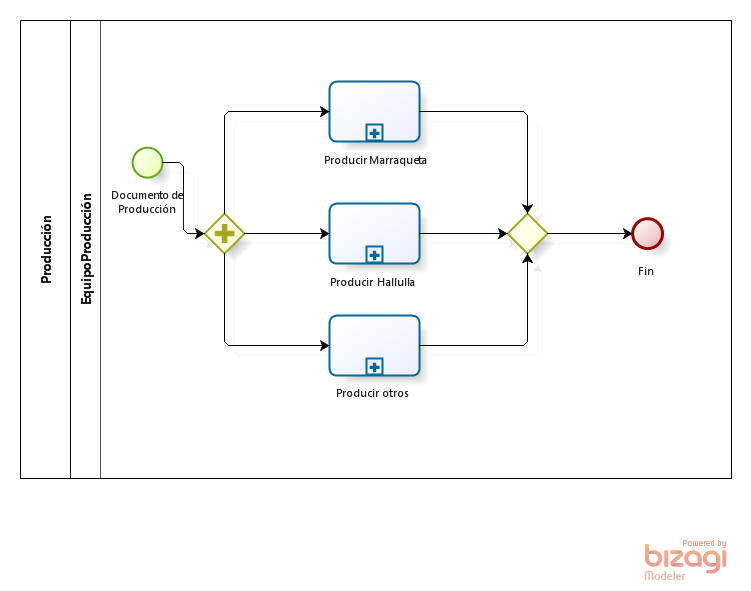
\includegraphics[width=13cm]{./imagenes/produccion_pan.png}\\
Figura 2: Proceso de producción de pan.
\end{center}

Se describir\'an los subprocesos Producci\'on de Hallulla y Producci\'on de Marraqueta, para modelar el proceso de producci\'on de pan:
\item \textbf{Producción de Hallulla:} Una de los 3 procesos más importantes de la panadería. Posee como entrada la solicitud de pedido del Proceso de Distribución. En este proceso actuan 4 personas con los siguientes roles:

\textbf{Actores:}
\begin{itemize}
\item Administrador: Encargado de recibir la solicitud y enviarla a Maestro panadero.
\item Maestro panadero: \item Maestro panadero: Encargado de recibir orden de pedido y entregarla al resto del equipo de producción de pan.
\item Oficiales: Encargado de la preparación de las latas, de cortar el pan, y enviarlo al enfriadero.
\item Hornero: Encargado de calentar el horno y de la cocción del pan.
\end{itemize} 

\begin{center}
\includegraphics[width=13cm]{./imagenes/Produccion_Hallulla.png}\\
Figura 3: Proceso de producción de pan Hallulla nivel 2.
\end{center}

\begin{center}
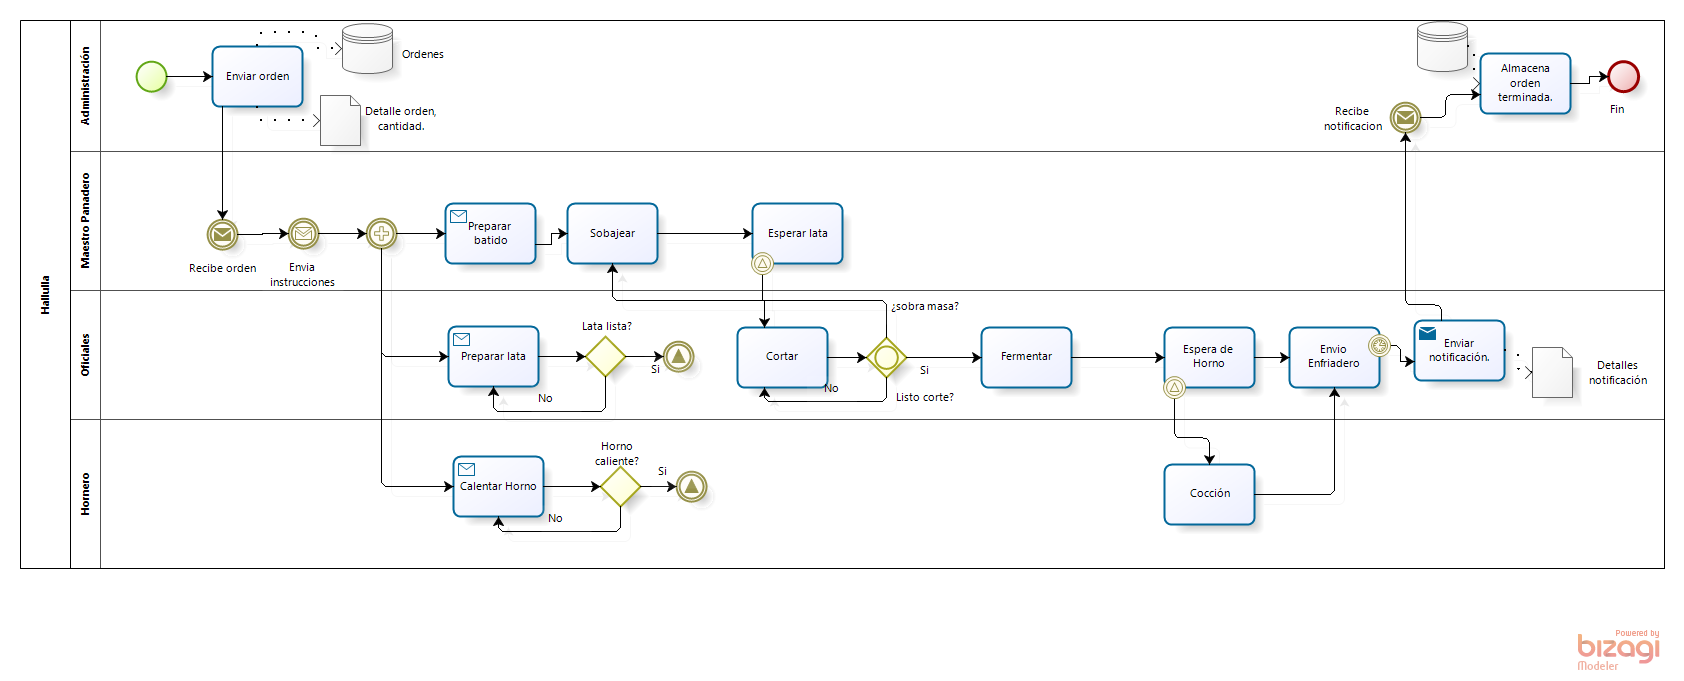
\includegraphics[width=13cm]{./imagenes/Produccion_HallullaNT.png}\\
Figura 4: Proceso de producción de pan Hallulla nivel 3.
\end{center}


\item \textbf{Producción de pan Marraqueta:}Uno de los 3 procesos más importantes de la panadería junto con el proceso descrito anterior. Al igual que el proceso de producción de pan Hallulla, posee como entrada la solicitud de pedido del Proceso de Distribución.

\textbf{Actores:}
\begin{itemize}
\item Administrador: Encargado de recibir la solicitud y enviarla a Maestro panadero.
\item Maestro panadero: \item Maestro panadero: Encargado de recibir orden de pedido y entregarla al resto del equipo de producción de pan.
\item Oficiales: Encargado de la preparación de las latas, de cortar el pan, y enviarlo al enfriadero.
\item Hornero: Encargado de calentar el horno y de la cocción del pan.
\end{itemize} 
\begin{center}
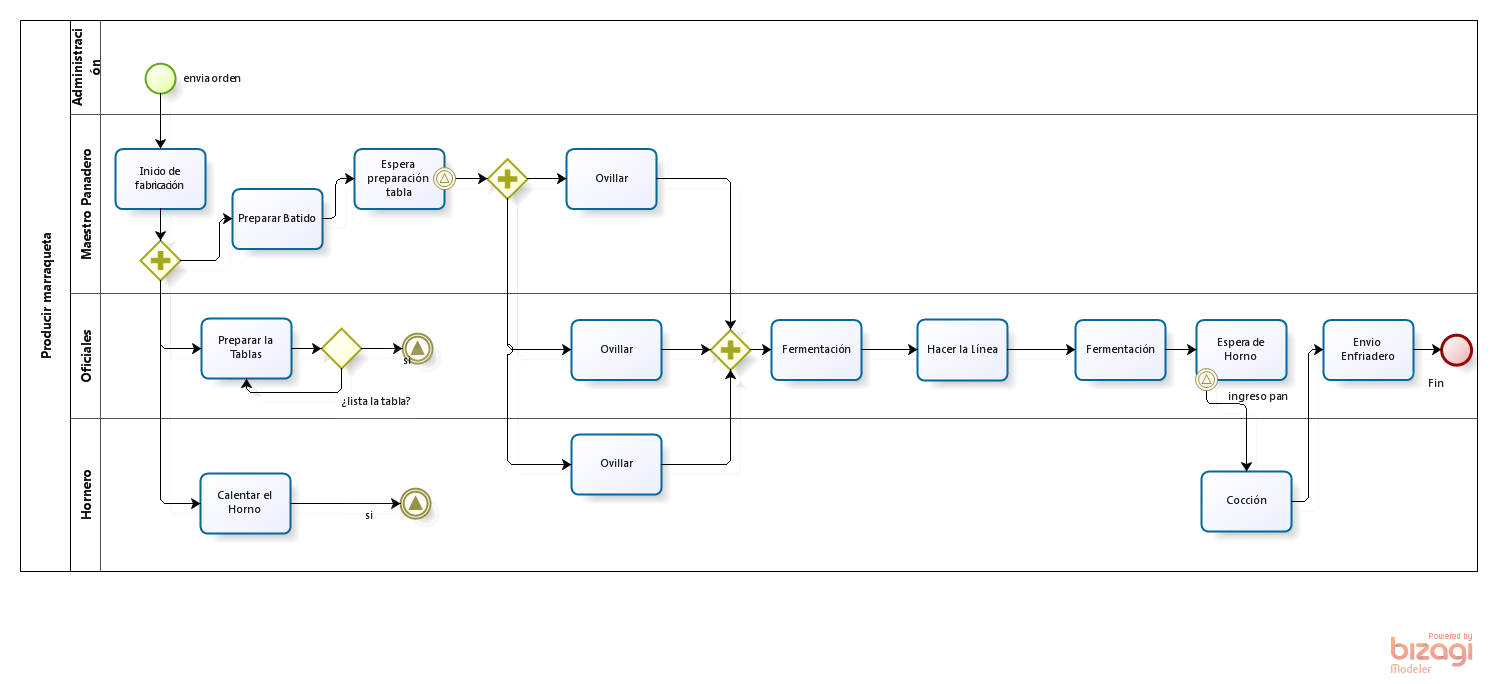
\includegraphics[width=13cm]{./imagenes/Produccion_Marraqueta.png}\\
Figura 5: Proceso de producción de pan  Marraquera nivel 2.
\end{center}

\begin{center}
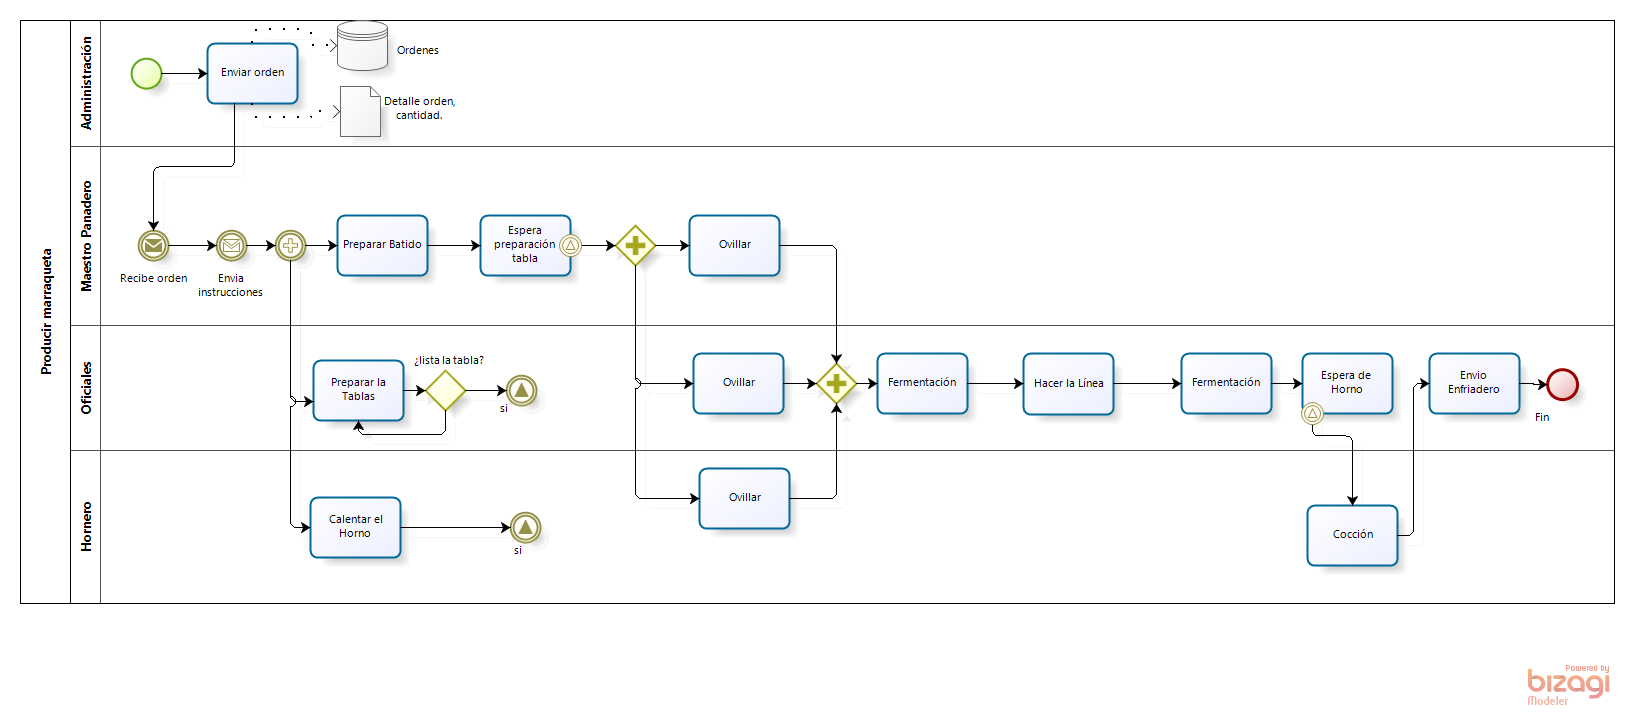
\includegraphics[width=13cm]{./imagenes/Produccion_MarraquetaNT.png}\\
Figura 6: Proceso de producción de pan  Marraquera nivel 3.
\end{center}

\item \textbf{Producción de repostería:} Se divide en 3 etapas que se hacen en paralelo pero no están sincronizados, Producir tortas, Producir galletas, Producir pasteles.

\begin{center}
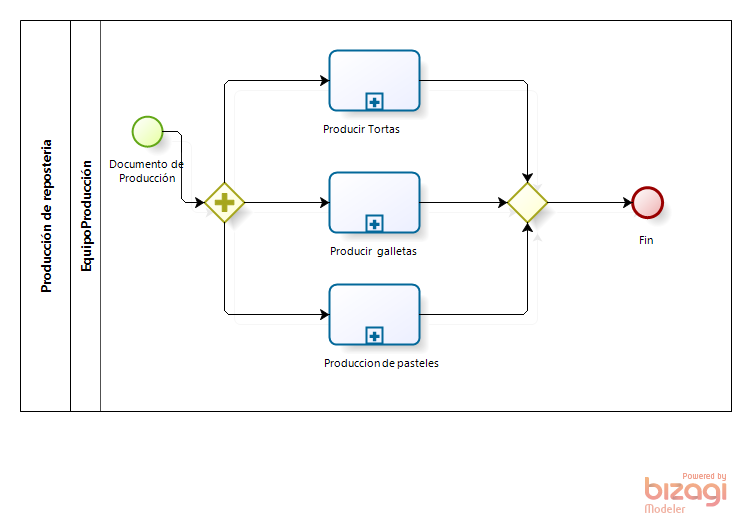
\includegraphics[width=13cm]{./imagenes/produccion_reposteria.png}\\
Figura 7: Proceso de producción de repostería.
\end{center}
Este proceso no fue modelado en los niveles operativos o tecnicos.
\item \textbf{Ventas:} El principal objetivo de este proceso es atender a la clientela, como punto de partida el cliente llega al local pidiendo el pan o repostería que quiere, se Recibe su pedido, luego se verifica si hay pan o repostería suficiente para atender lo requerido, puede haber o no, en caso de no haber pan o repostería se ve cuanta cantidad se necesitaría aproximadamente y se envía a Producción, en este último pueden hacer más pan o repostería o simplemente notifican que no se puede hacer más pan por motivos varios, en caso de hacer más pan o repostería se envía pan o repostería a la sala de ventas, se hace el vale. Ahora en caso de que haya pan o repostería solamente se procede a hacer el vale. Luego el cliente recibe el vale con el cual procede a pagar finalizando el proceso.

\textbf{Actores:}
\begin{itemize}
\item Vendedora: La vendedora es la encargada de recibir al cliente que llega, recibe el pedido y revisa si hay stock de pan o repostería en ese momento, en caso contrario pide en la fábrica más pan o repostería, además es la encargada de hacer el vale para posteriormente el cliente pague.
\item Cajera: Es la encargada de cobrar el dinero al cliente
\item Cliente: El más importante dentro de este proceso, es quien hace el pedido y quien debe pagar por aquello además de recibir el vale por supuesto.
\end{itemize} 

\begin{center}
\includegraphics[width=15cm]{./imagenes/Proceso_VentasN1.png}\\
Figura 8: Proceso de Ventas.
\end{center}


\begin{center}
\includegraphics[width=15cm]{./imagenes/Proceso_VentasN2.png}\\
Figura 9: Proceso de Ventas nivel 2.
\end{center}


\begin{center}
\includegraphics[width=15cm]{./imagenes/Proceso_VentasN3.png}\\
Figura 10: Proceso de Ventas nivel 3.
\end{center}


\item \textbf{Distribución:} Este proceso se encarga a grandes rasgos de enviar el pedido a los distintos locales, ya sea en la zona como en los alrededores. Todo empieza por recibir el pedido, luego se aprueba la solicitud para después ver si se acepta el pedido o no. Aceptar el pedido implica que se debe mandar la cantidad que pide el cliente, esto se denomina hacer las cargas, en caso contrario se disminuye la cantidad y se hace las cargas. Paralelamente se comprueban las cargas y se registran para luego proceder al reparto, una vez en el lugar se ve si se cobra o no, en caso de cobrar el cliente debe pagar la cantidad predefinida, en caso contrario es porque el cliente paga mensualmente el pan distribuido. Finalmente se recauda el dinero dando término al proceso.

\textbf{Actores:} 
\begin{itemize}
\item Administrador: Persona que ve si realmente se aprueba la solicitud del cliente, es capaz de modificar el pedido en caso que el cliente devuelva pan, también comprueba las cargas y registra el reparto para tener un control de aquello y finalmente recauda el dinero del reparto
\item Repartidor: Es quien recibe el pedido, hace las cargas, reparte a los distintos locales y a veces, dependiendo de cual sea el caso, le toca cobrar a los clientes directamente.
\item Cliente: Es aquel que tiene un negocio o local y necesita de pan para atender a su propia clientela, solicita un pedido y a la hora de llegar puede pagarlo en el momento o simplemente pagarlo a final de mes.
\end{itemize}

\begin{center}
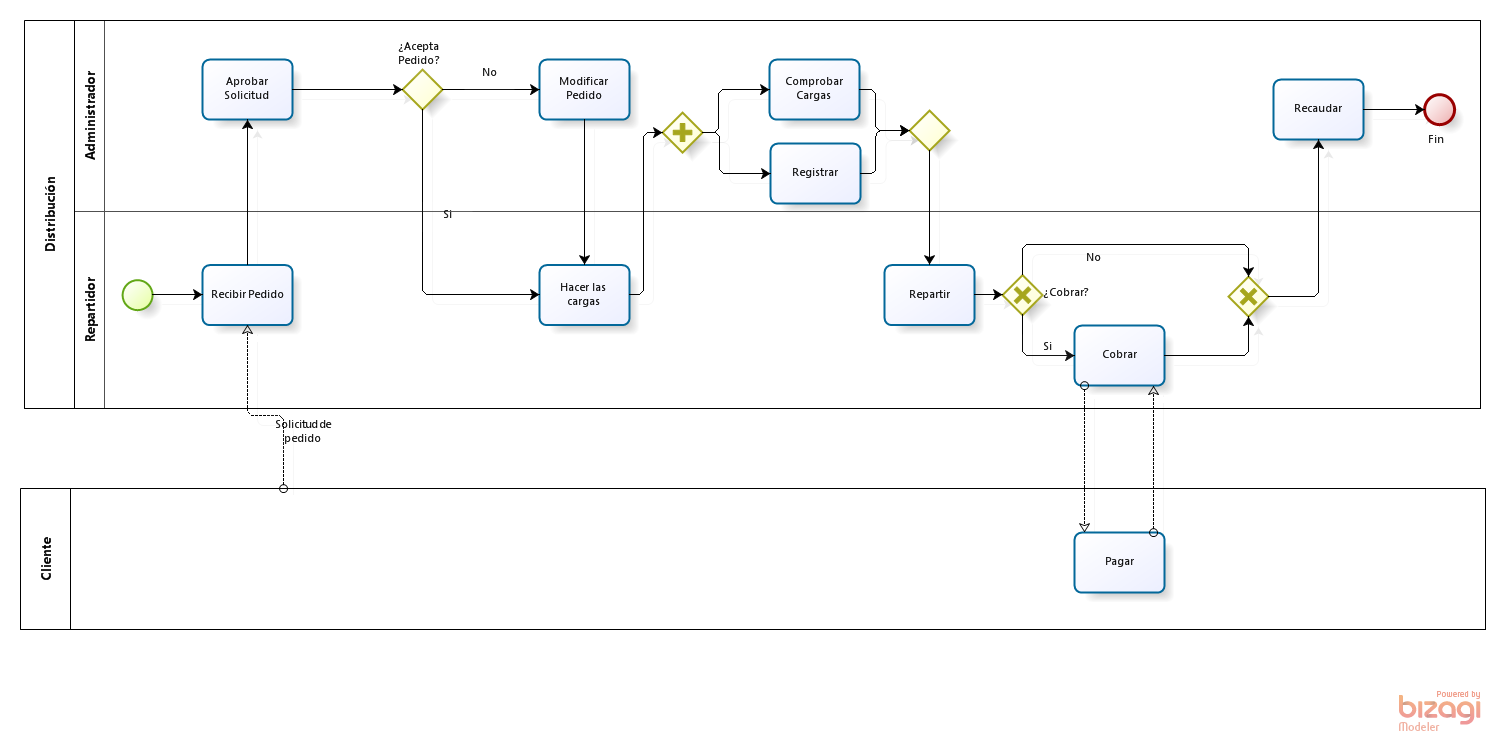
\includegraphics[width=15cm]{./imagenes/Distribucion.png}\\
Figura 11: Proceso de Distribución.
\end{center}

\begin{center}
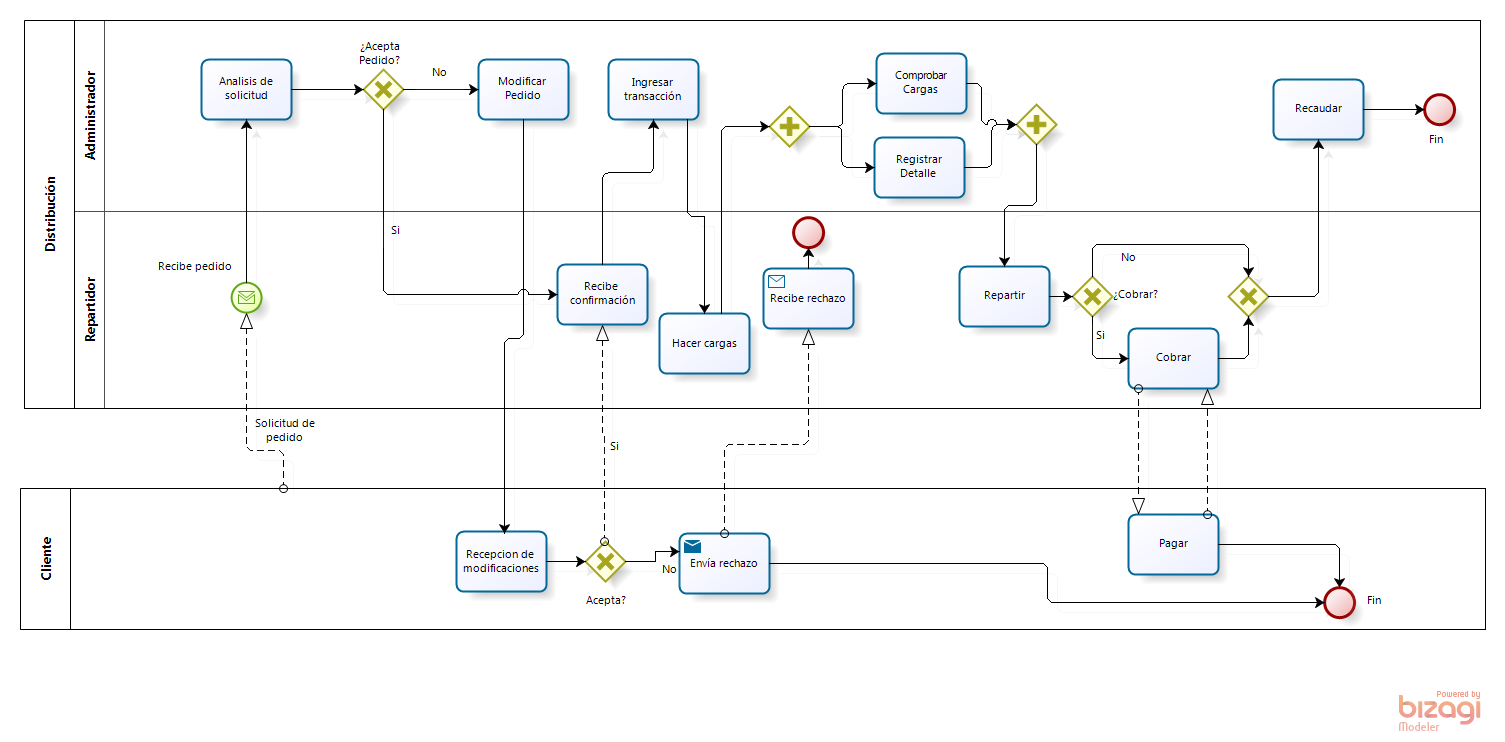
\includegraphics[width=15cm]{./imagenes/DistribucionN2.png}\\
Figura 12: Proceso de Distribución nivel 2.
\end{center}

\begin{center}
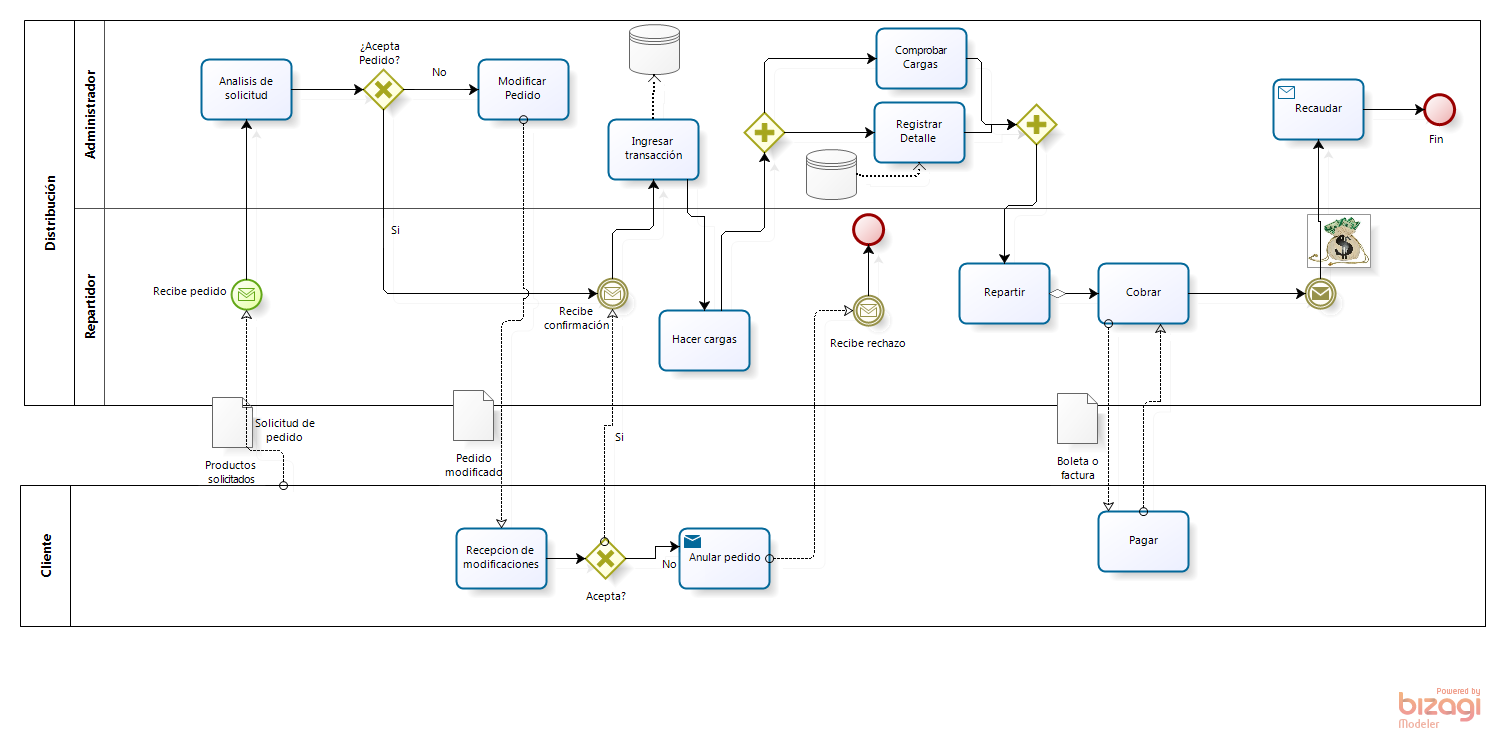
\includegraphics[width=15cm]{./imagenes/DistribucionN3.png}\\
Figura 13: Proceso de Distribución nivel 3.
\end{center}


\item \textbf{Abastecimiento:}
Este proceso es necesario para el abastecimiento del local comercial, con el fin de producir los productos necesarios, como pan, torta, pasteles y/o galletas. Todo comienza cuando el administrador recibe el pedido de parte del área de producción al no poseer los insumos necesarios para producir, posteriormente se evalúa si existe el stock para cubrirlo, si es posible, se entregan al área de producción, si no se debe cuantificar lo que falta, elegir el proveedor al que se debe enviar el pedido y finalmente enviar la solicitud. Cuando esto ocurre, el proveedor recibe el pedido, genera la factura la cual es enviada al administrador que paga lo solicitado, para luego recibir los insumos y entregarlos al área de producción.

\textbf{Actores:} 
\begin{itemize}
\item Administrador: Persona que recibe pedido y se encarga de comprar los insumos necesarios para luego entregarlos al área de producción.
\item Proveedor: Aquello que proporciona el pedido solicitado.
\end{itemize}

\begin{center}
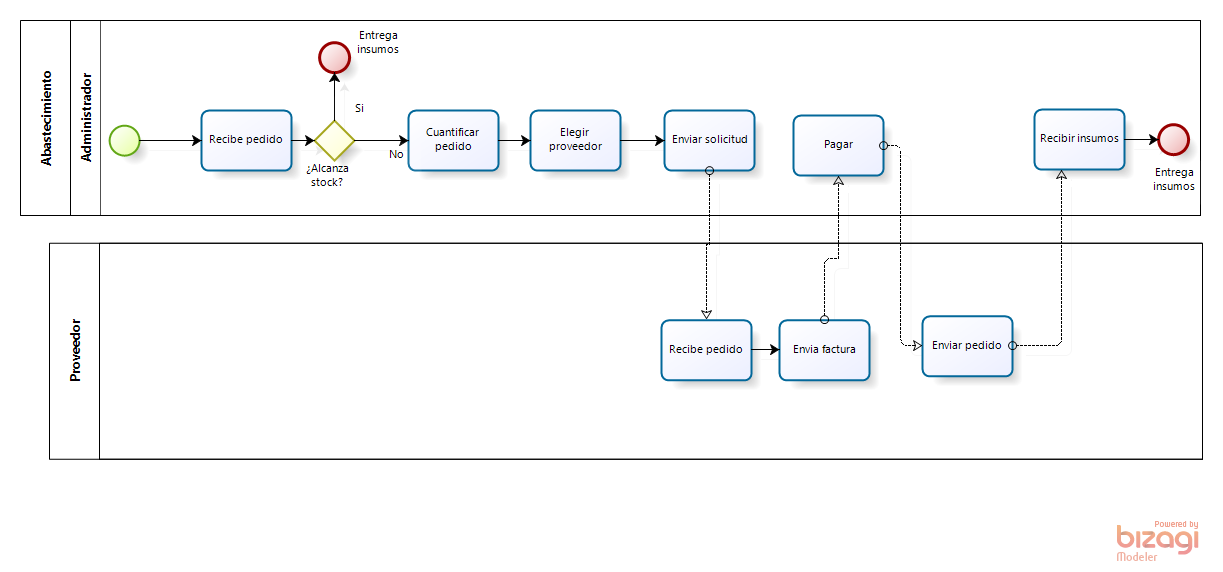
\includegraphics[width=15cm]{./imagenes/Abastecimiento.png}\\
Figura 14: Proceso de Abastecimiento.
\end{center}

\begin{center}
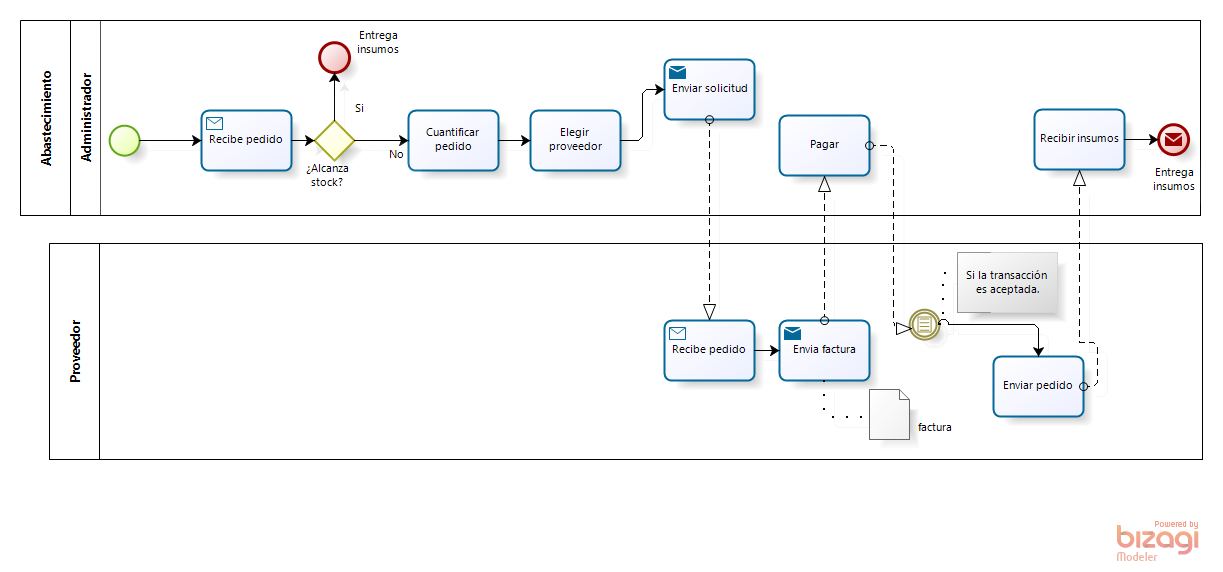
\includegraphics[width=15cm]{./imagenes/AbastecimientoN2.png}\\
Figura 15: Proceso de Abastecimiento de nivel 2.
\end{center}

\begin{center}
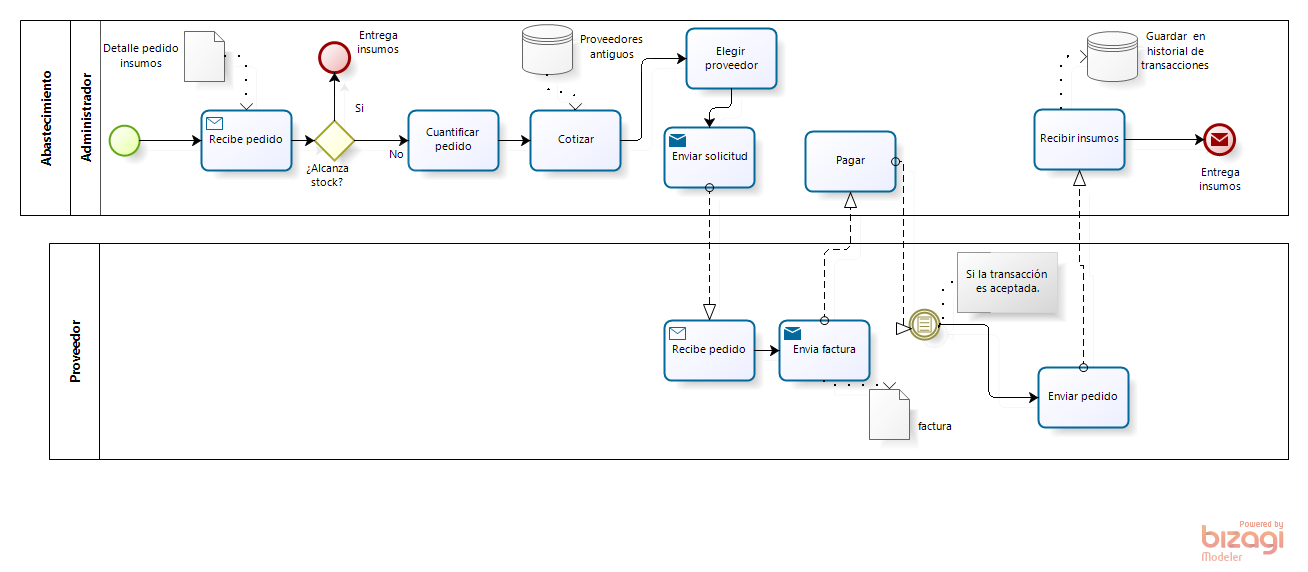
\includegraphics[width=15cm]{./imagenes/AbastecimientoNT.png}\\
Figura 16: Proceso de Abastecimiento de nivel 3.
\end{center}

\end{itemize}
